%% TODO reemplazar y verificar el uso de "el video de boca". Como hacemos para reemplazarlo??
\section{Comparación con IFTrace}

El algoritmo de seguimiento IFTrace, propuesto por \citeauthor*{IFTrace}, es un algoritmo robusto que soporta
cambios de iluminación y forma, oclusiones y se centra en hallar características representativas de la textura
de los objetos a seguir. Es capaz de recuperarse de errores menores y permite el seguimiento de múltiples objetos
a la vez.

\begin{figure}[H]
    \label{fig:happy-occluded-iftrace}
    \centering
    \begin{tabular}{cccc}
        \subfloat{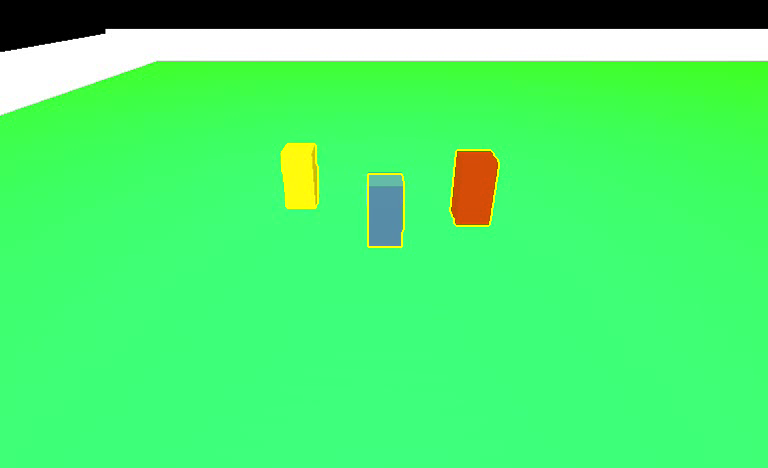
\includegraphics[width = 1.5in]{./images/happy_occluded_00001.png}} &
        \subfloat{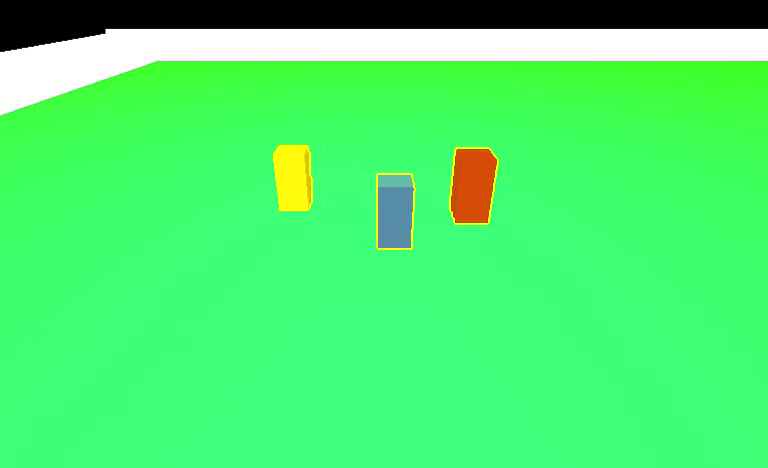
\includegraphics[width = 1.5in]{./images/happy_occluded_00003.png}} &
        \subfloat{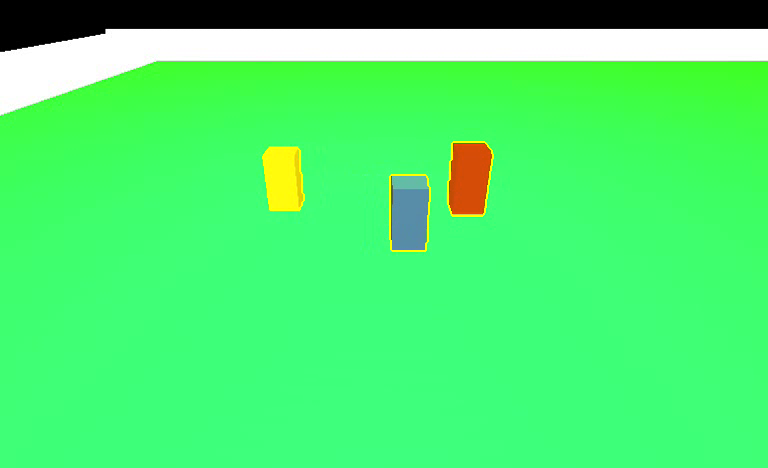
\includegraphics[width = 1.5in]{./images/happy_occluded_00005.png}} &
        \subfloat{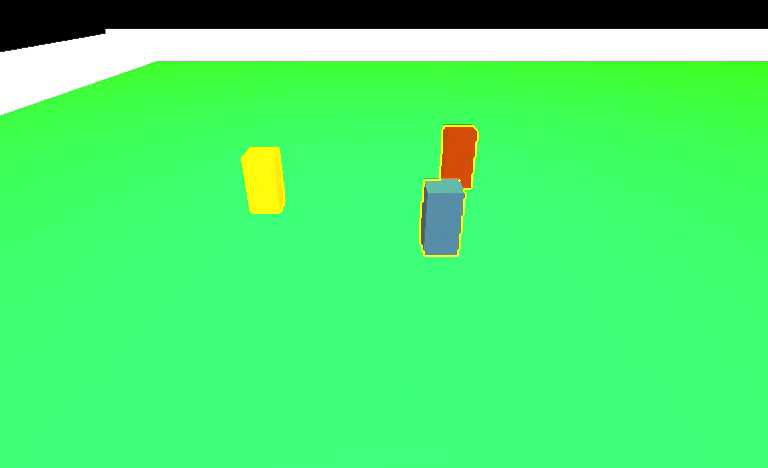
\includegraphics[width = 1.5in]{./images/happy_occluded_00008.png}}
    \end{tabular}
    \caption{IFTrace funcionando en una secuencia de cuadros de video sintético.}
\end{figure}

Un algoritmo de este tipo podría proporcionar una buena solución a nuestro problema. Como se puede ver en la figura
\ref{fig:happy-occluded-iftrace}, IFTrace logra un correcto seguimiento de múltiples objetos simples de diferentes características.
También puede observarse, en la figura \ref{fig:boca-iftrace}, como sigue correctamente a un jugador en un video de fútbol real. Desafortunadamente,
el algoritmo no logra seguirlo correctamente por más de unos pocos cuadros, cayendo en un error del cual sólo una corrección manual
puede sacarlo. Este tipo de correción supervisada no está contemplada en el algoritmo de IFTrace.

\begin{figure}[H]
    \label{fig:boca-iftrace}
    \centering
    \begin{tabular}{cccc}
        \subfloat{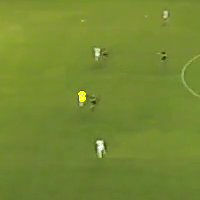
\includegraphics[width = 1.5in]{./images/cropped_boca_00009}} &
        \subfloat{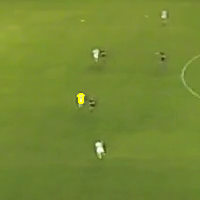
\includegraphics[width = 1.5in]{./images/cropped_boca_00012}} &
        \subfloat{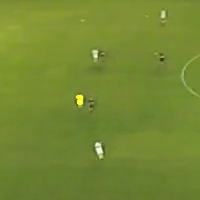
\includegraphics[width = 1.5in]{./images/cropped_boca_00014}} &
        \subfloat{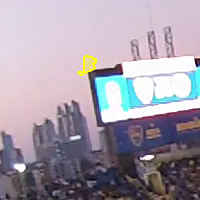
\includegraphics[width = 1.5in]{./images/cropped_boca_00017}}
    \end{tabular}
    \caption{Seguimiento de un jugador en un video real utilizando IFTrace.}
\end{figure}

%TODO Meter aca 4 cuadros mostrando como nuestro algoritmo funciona. Deberian ser los mismos.

Como se puede observar en las figuras \ref{fig:happy-occluded-activeContour} y \ref{fig:boca-activeContour}, nuestro algoritmo
sigue con exito a los objetos de interés.

\subsection{Performance}

Otro punto importante de comparación entre los dos algoritmos es su tiempo de ejecución, es decir el tiempo que tarda en llevar a cabo su trabajo.
De acuerdo a nuestras mediciones, realizadas con un video real de un partido de fútbol, siguiendo a un solo jugador, el tiempo promedio que
tarda IFTrace por cuadro es 6.962 segundos, mientras que nuestro algoritmo tiene un tiempo promedio de 0.700 segundos. Se puede observar que
%% 6.9628571428571435 si quieren los decimales
%% TODO verificar nuestro numero!!!
se encuentra un orden magnitud por debajo de IFTrace.

Cabe destacar que ambos algoritmos podrían verse beneficiados por numerosas optimizaciones, como por ejemplo en el caso de IFTrace la programación
en GPU. Sin embargo, por razones de practicidad se tomaron estas mediciones con versiones estándar de ambos algoritmos.

- Performance con videos de ellos. Performance con nuestro video DONE!
- Performance con video sintético DONE!
- Comparación de nuestros resultados vs los de ellos (Métrica: cantidad de jugadores perdidos por frame -- o si se nos ocurre una mejor ambas o esa)
